%%%%%%%%%%%%%%%%%%%%%%%%%%%%
%%  Componenti del front end
%%%%%%%%%%%%%%%%%%%%%%%%%%%%



\subsection{\nogloxy{swedesigner::client}}
\label{\nogloxy{swedesigner::client}}
\subsubsection{Informazioni generali}
\begin{itemize}
\item \textbf{Descrizione}\\
Questo package descrive le componenti del \emph{front end}, scritte in JavaScript.
\item \textbf{Padre}: \hyperref[\nogloxy{swedesigner}]{\nogloxy{\texttt{swedesigner}}}
\item \textbf{Package contenuti}:
\begin{itemize}
\item \hyperref[\nogloxy{swedesigner::client::collection}]{\nogloxy{\texttt{collection}}}\\
Questo package descrive le classi che contengono delle collection (secondo la visione di \backbonejs). 
\item \hyperref[\nogloxy{swedesigner::client::model}]{\nogloxy{\texttt{model}}}\\
Questo package contiene i modelli di dati usati dal client per rappresentare l'informazione manipolata dall'utente.
\item \hyperref[\nogloxy{swedesigner::client::view}]{\nogloxy{\texttt{view}}}\\
Questo package raccoglie le classi che rappresentano i menù laterali e il \texttt{canvas} visualizzati dal browser, che popolano template e si sottoscrivono alla view tramite un pattern Observer. (I template non sono contenuti in questo package.)
\end{itemize}
\end{itemize}

\subsection{\nogloxy{swedesigner::client::collection}}
\label{\nogloxy{swedesigner::client::collection}}
\subsubsection{Informazioni generali}
\begin{itemize}
\item \textbf{Descrizione}\\
Questo package descrive le classi che contengono delle collection (secondo la visione di \backbonejs).
\item \textbf{Padre}: \hyperref[\nogloxy{swedesigner::client}]{\nogloxy{\texttt{client}}}
\end{itemize}

\subsection{\nogloxy{swedesigner::client::model}}
\label{\nogloxy{swedesigner::client::model}}
\subsubsection{Informazioni generali}
\begin{adjustwidth}{-3cm}{-3cm}

\begin{figure}[H]
\centering
\nogloxy{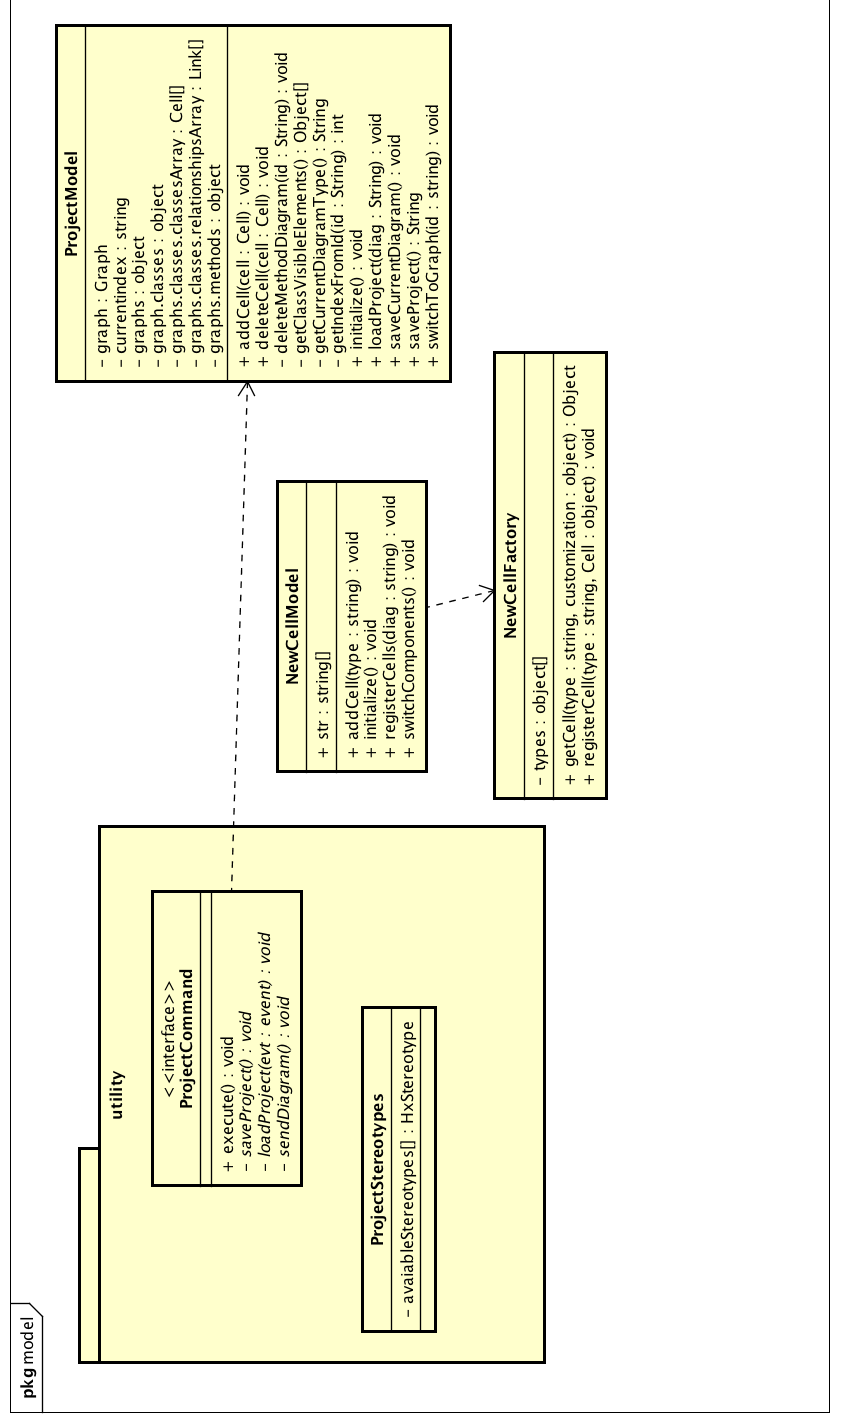
\includegraphics[scale=0.5,keepaspectratio]{img/client/model_pkg.png}}
\caption{\nogloxy{swedesigner::client::model}}
\end{figure}

\end{adjustwidth}

\FloatBarrier
\begin{itemize}
\item \textbf{Descrizione}\\
Questo package contiene i modelli di dati usati dal client per rappresentare l'informazione manipolata dall'utente.
\item \textbf{Padre}: \hyperref[\nogloxy{swedesigner::client}]{\nogloxy{\texttt{client}}}
\item \textbf{Package contenuti}:
\begin{itemize}
\item \hyperref[\nogloxy{swedesigner::client::model::celltypes}]{\nogloxy{\texttt{celltypes}}}\\
Questo package contiene la definizione del modello degli elementi grafici dell'applicazione (e.g. diagrammi delle classi, blocchi condizionali\dots). 
\item \hyperref[\nogloxy{swedesigner::client::model::utility}]{\nogloxy{\texttt{utility}}}\\
Questo package racchiude le classi che definiscono i principali comandi dell'applicazione; esse fanno parte di un unico pattern Command, usato dalla \texttt{AppView} principale.
\end{itemize}
\end{itemize}
\subsubsection{Classi}
\subsubsubsection{\nogloxy{swedesigner::client::model::NewCellFactory}}
\label{\nogloxy{swedesigner::client::model::NewCellFactory}}
\begin{itemize}
\item \textbf{Descrizione}\\
questa classe si occupa di fornire un'istanza di una cella del tipo richiesto da \texttt{NewCellModel}. 
\item \textbf{Utilizzo}\\
viene utilizzata da \texttt{NewCellModel} che richiede una nuova cella (blocco o relazione) per avere un'istanza del blocco richiesto. Il design pattern descritto da questa classe è un Factory Pattern, come spiegato nel libro \emph{Learning Javascript Design Patterns} (\url{addyosmani.com/resources/essentialjsdesignpatterns/book/}).
\item \textbf{Relazioni con altre classi}:
\begin{itemize}
\item \textit{IN} \hyperref[\nogloxy{swedesigner::client::model::celltypes::activity::ActivityDiagramElement}]{\nogloxy{\texttt{ActivityDiagramElement}}}\\
questa classe è la base di tutte le classi che rappresentano i blocchi del diagramma delle attività.
\item \textit{IN} \hyperref[\nogloxy{swedesigner::client::model::NewCellModel}]{\nogloxy{\texttt{NewCellModel}}}\\
questa classe si occupa di fornire tutti i tipi di cell (tutti i blocchi e relazioni) da poter inserire nel diagramma corrente (o classi o attività).
\item \textit{OUT} \hyperref[\nogloxy{swedesigner::client::model::celltypes::class::ClassDiagramElement}]{\nogloxy{\texttt{ClassDiagramElement}}}\\
questa classe è la base di tutte le classi che rappresentano gli elementi del diagramma delle classi.
\end{itemize}
\item \textbf{Attributi}:
\begin{itemize}
\item \nogloxy{\texttt{- types: object[]}}
\\ Questo attributo indica l'array che verrà utilizzato per salvare i tipi di celle delle quali ritornare un'istanza quando richiesto
\end{itemize}
\item \textbf{Metodi}:
\begin{itemize}
\item \nogloxy{\texttt{+ getCell(type: string, customization: object): object}}
\\ Questo metodo ritorna un istanza della cella del tipo specificato
\\ \textbf{Parametri}:
\begin{itemize}
\item \nogloxy{\texttt{type: string}}
\\ Questo parametro indica il tipo della cella della quale si richiede un'istanza
\item \nogloxy{\texttt{customization: object}}
\\ Questo parametro indica delle proprietà aggiuntive da poter aggiungere all'istanza della cella richiesta
\end{itemize}
\item \nogloxy{\texttt{+ registerCell(type: string, Cell: object): void}}
\\ Questo metodo permette di registrare nella factory una nuova cella
\\ \textbf{Parametri}:
\begin{itemize}
\item \nogloxy{\texttt{type: string}}
\\ Questo parametro indica il nome con cui verrà identificata la cella nella factory
\item \nogloxy{\texttt{Cell: object}}
\\ Questo parametro indica il prototipo della cella che verrà usato per creare le istanze
\end{itemize}
\end{itemize}
\end{itemize}

\subsubsubsection{\nogloxy{swedesigner::client::model::NewCellModel}}
\label{\nogloxy{swedesigner::client::model::NewCellModel}}
\begin{itemize}
\item \textbf{Descrizione}\\
questa classe si occupa di fornire tutti i tipi di cell (tutti i blocchi e relazioni) da poter inserire nel diagramma corrente (o classi o attività).
\item \textbf{Utilizzo}\\
utilizza \texttt{NewCellFactory} per recuperare una cell del tipo richiesto da \texttt{NewCellView}. Quest'ultima utilizza \texttt{NewCellModel} come modello da dove recuperare tutti i blocchi/relazioni che l'utente può inserire nel diagramma corrente.
\item \textbf{Relazioni con altre classi}:
\begin{itemize}
\item \textit{IN} \hyperref[\nogloxy{swedesigner::client::view::NewCellView}]{\nogloxy{\texttt{NewCellView}}}\\
questa classe si occupa di visualizzare tutti i possibili blocchi e relazioni che si possono inserire nel diagramma delle classi o delle attività.
\item \textit{OUT} \hyperref[\nogloxy{swedesigner::client::model::NewCellFactory}]{\nogloxy{\texttt{NewCellFactory}}}\\
questa classe si occupa di fornire un'istanza di una cella del tipo richiesto da \texttt{NewCellModel}. 
\end{itemize}
\item \textbf{Attributi}:
\begin{itemize}
\item \nogloxy{\texttt{- str: string[]}}
\\ Questo attributo indica l'elenco dei blocchi disponibili in base al diagramma corrente
\end{itemize}
\item \textbf{Metodi}:
\begin{itemize}
\item \nogloxy{\texttt{+ addCell(type: string): void}}
\\ Questo metodo richiede una nuova istanza della cella richiesta e la passa a \texttt{ProjectModel}
\\ \textbf{Parametri}:
\begin{itemize}
\item \nogloxy{\texttt{type: string}}
\\ Questo parametro indica il tipo di cella della quale si richiede l'istanza
\end{itemize}
\item \nogloxy{\texttt{+ initialize(): void}}
\\ Questo metodo si occupa di inizializzare la classe e richiamare la funzione di aggiornamento dell'elenco dei blocchi disponibili
\item \nogloxy{\texttt{+ registerCells(diag: string): void}}
\\ Questo metodo si occupa di aggiornare i blocchi disponibili in base al diagramma corrente
\\ \textbf{Parametri}:
\begin{itemize}
\item \nogloxy{\texttt{diag: string}}
\\ Questo parametro indica il tipo del diagramma corrente
\end{itemize}
\item \nogloxy{\texttt{+ switchComponents(): void}}
\\ Questo metodo si occupa di richiamare l'aggiornamento dei blocchi disponibile quando viene cambiato il tipo di diagramma
\end{itemize}
\end{itemize}

\subsubsubsection{\nogloxy{swedesigner::client::model::ProjectCommand}}
\label{\nogloxy{swedesigner::client::model::ProjectCommand}}
\begin{itemize}
\item \textbf{Descrizione}\\
questa interfaccia descrive la struttura di un comando che viene chiamato da \texttt{AppView} quando l'utente decide di creare un nuovo progetto, di caricarne uno esistente, di salvarlo o di generare il codice dal diagramma. Il pattern realizzato è il pattern Command.
\item \textbf{Utilizzo}\\
viene utilizzata da \texttt{AppView}, la quale poi chiederà comandi concreti in base all'input richiesto dall'utente.
\item \textbf{Relazioni con altre classi}:
\begin{itemize}
\item \textit{IN} \hyperref[\nogloxy{swedesigner::client::view::AppView}]{\nogloxy{\texttt{AppView}}}\\
questa classe si occupa di gestire l'intera view dell'applicazione, componendo l'interfaccia principale e richiamando le altre view tramite il sistema a template di \backbonejs{}.
\item \textit{OUT} \hyperref[\nogloxy{swedesigner::client::model::ProjectModel}]{\nogloxy{\texttt{ProjectModel}}}\\
questa classe ci permette di aggiungere della logica alla collezione di tutti i diagrammi che possediamo.
\end{itemize}
\item \textbf{Metodi}:
\begin{itemize}
\item \nogloxy{\texttt{+ execute(name: string, [*args]: array): function}}
\\ Questo metodo permette di eseguire un metodo all'interno di ProjectCommand in base al nome passato come parametro
\\ \textbf{Parametri}:
\begin{itemize}
\item \nogloxy{\texttt{name: string}}
\\ Questo parametro indica il nome del metodo che si vuole eseguire
\item \nogloxy{\texttt{[*args]: array}}
\\ È possibile inserire una serie di parametri aggiuntivi da poter passare alle funzioni richiamate
\end{itemize}
\item \nogloxy{\texttt{+ loadDiagram(evt: object): void}}
\\ Questo metodo si occupa di prendere in input un progetto in formato json e caricarlo nell'editor
\\ \textbf{Parametri}:
\begin{itemize}
\item \nogloxy{\texttt{evt: object}}
\\ Questo parametro indica un oggetto che rappresenta l'evento di un campo input type file di html
\end{itemize}
\item \nogloxy{\texttt{+ saveDiagram(): void}}
\\ Questo metodo si occupa di fornire il comando per salvare in locale il progetto in formato json
\item \nogloxy{\texttt{+ sendDiagram(): void}}
\\ Questo metodo si occupa di inviare al server il progetto e scaricare il codice generato
\end{itemize}
\end{itemize}

\subsubsubsection{\nogloxy{swedesigner::client::model::ProjectModel}}
\label{\nogloxy{swedesigner::client::model::ProjectModel}}
\begin{itemize}
\item \textbf{Descrizione}\\
questa classe ci permette di aggiungere della logica alla collezione di tutti i diagrammi che possediamo.
\item \textbf{Utilizzo}\\
essa è istanziata da \texttt{ProjectView} e possiede \texttt{DiagramCollection}. È possibile interagire con questo modello anche tramite \texttt{ProjectCommand}, per permettere l'implementazione di funzionalità globali dell'applicazione (e.g. salvataggio e caricamento).
\item \textbf{Relazioni con altre classi}:
\begin{itemize}
\item \textit{IN} \hyperref[\nogloxy{swedesigner::client::model::ProjectCommand}]{\nogloxy{\texttt{ProjectCommand}}}\\
questa interfaccia descrive la struttura di un comando che viene chiamato da \texttt{AppView} quando l'utente decide di creare un nuovo progetto, di caricarne uno esistente, di salvarlo o di generare il codice dal diagramma. Il pattern realizzato è il pattern Command.
\item \textit{IN} \hyperref[\nogloxy{swedesigner::client::view::AppView}]{\nogloxy{\texttt{AppView}}}\\
questa classe si occupa di gestire l'intera view dell'applicazione, componendo l'interfaccia principale e richiamando le altre view tramite il sistema a template di \backbonejs{}.
\item \textit{IN} \hyperref[\nogloxy{swedesigner::client::view::ProjectView}]{\nogloxy{\texttt{ProjectView}}}\\
questa classe rappresenta l'area di disegno principale dell'applicazione, che necessita di essere cambiata tra diagramma delle classi e diagramma delle attività. 
\end{itemize}
\item \textbf{Attributi}:
\begin{itemize}
\item \nogloxy{\texttt{- currentIndex: String}}
\\ Rappresenta l'identificativo del diagramma corrente che può essere "class" in caso del diagramma delle classi o un id univoco in caso di un diagramma delle attività
\item \nogloxy{\texttt{- graph: Graph}}
\\ Rappresenta il model utilizzato per contenere tutte le celle del diagramma corrente.
\item \nogloxy{\texttt{- graphs: Object}}
\\ Contiene al suo interno la struttura dati scollegata dalla rappresentazione di \jointjs{} e utilizzata per l'invio dei dati al server.
\item \nogloxy{\texttt{- graphs.classes: Object}}
\\ Contiene gli elementi che rappresentano le classi del progetto.
\item \nogloxy{\texttt{- graphs.classes.classesArray: Cell[]}}
\\ Contiene l'array di elementi usati per rappresentare le classi del diagramma delle classi.
\item \nogloxy{\texttt{- graphs.classes.relationshipsArray: Link[]}}
\\ Contiene l'array di elementi usati per rappresentare le relazioni del diagramma delle classi.	

\item \nogloxy{\texttt{- graphs.methods: object}}
\\ Contiene l'array  di oggetti che rappresentano ognuno un diagramma delle attività
\end{itemize}
\item \textbf{Metodi}:
\begin{itemize}
\item \nogloxy{\texttt{+ addCell(cell: Cell): void}}
\\ Aggiunge una cella generica passata in input al diagramma corrente.
\\ \textbf{Parametri}:
\begin{itemize}
\item \nogloxy{\texttt{cell: Cell}}
\\ Questo parametro indica l'istanza della cella da aggiungere al diagramma corrente
\end{itemize}
\item \nogloxy{\texttt{+ deleteCell(cell: Cell): void}}
\\ Cancella la cella passata come parametro dal diagramma corrente. Se è una cella di una classe o di una interfaccia cancella anceh i relativi diagrammi delle attività.
\\ \textbf{Parametri}:
\begin{itemize}
\item \nogloxy{\texttt{cell: Cell}}
\\ Cella da rimuovere.
\end{itemize}
\item \nogloxy{\texttt{- deleteMethodDiagram(id: String): void}}
\\ Rimuove il diagramma delle attività specificato in input.
\\ \textbf{Parametri}:
\begin{itemize}
\item \nogloxy{\texttt{id: String}}
\\ Id del diagramma delle attività da rimuovere.
\end{itemize}
\item \nogloxy{\texttt{- getClassVisibleElements(): Object[]}}
\\ Ritorna un array composto da elementi con attributi \emph{label} pari e \emph{value}. Questo array rappresenta i metodi e gli attributi visibili da un metodo( solo di quella classe) che verranno suggeriti all'utente durante la costruzione del diagramma delle attività
\item \nogloxy{\texttt{- getCurrentDiagramType(): String}}
\\ Ritorna il tipo corrente di diagramma selezionato.
\item \nogloxy{\texttt{- getIndexFromId(id: String): int}}
\\ Ritorna l'indice del diagramma a partire dall'id passato in input.
\\ \textbf{Parametri}:
\begin{itemize}
\item \nogloxy{\texttt{id: String}}
\\ Id del diagramma.
\end{itemize}
\item \nogloxy{\texttt{+ initialize(): void}}
\\ Assegna una nuova istanza di Graph a graph appropriata.
\item \nogloxy{\texttt{+ loadProject(diag: String): void}}
\\ Carica il progetto passato in input.
\\ \textbf{Parametri}:
\begin{itemize}
\item \nogloxy{\texttt{diag: String}}
\\ Progetto in formato JSON.
\end{itemize}
\item \nogloxy{\texttt{+ saveCurrentDiagram(): void}}
\\ Salva all'interno di graphs il diagramma corrente.
\item \nogloxy{\texttt{+ saveProject(): String}}
\\ Ritorna l'intero progetto in formato JSON. % e allora chiamiamolo magari saveProject
\item \nogloxy{\texttt{+ switchToGraph(id: string): void}}
\\ Salva il diagramma corrente e ne carica un'altro in base all'input
\\ \textbf{Parametri}:
\begin{itemize}
\item \nogloxy{\texttt{id: string}}
\\ Questo parametro indica l'id del diagramma al quale si vuole passare
\end{itemize}
\end{itemize}
\end{itemize}
\subsection{\nogloxy{swedesigner::client::model::celltypes}}
\label{\nogloxy{swedesigner::client::model::celltypes}}
\subsubsection{Informazioni generali}
\begin{figure}[h]
\centering
\nogloxy{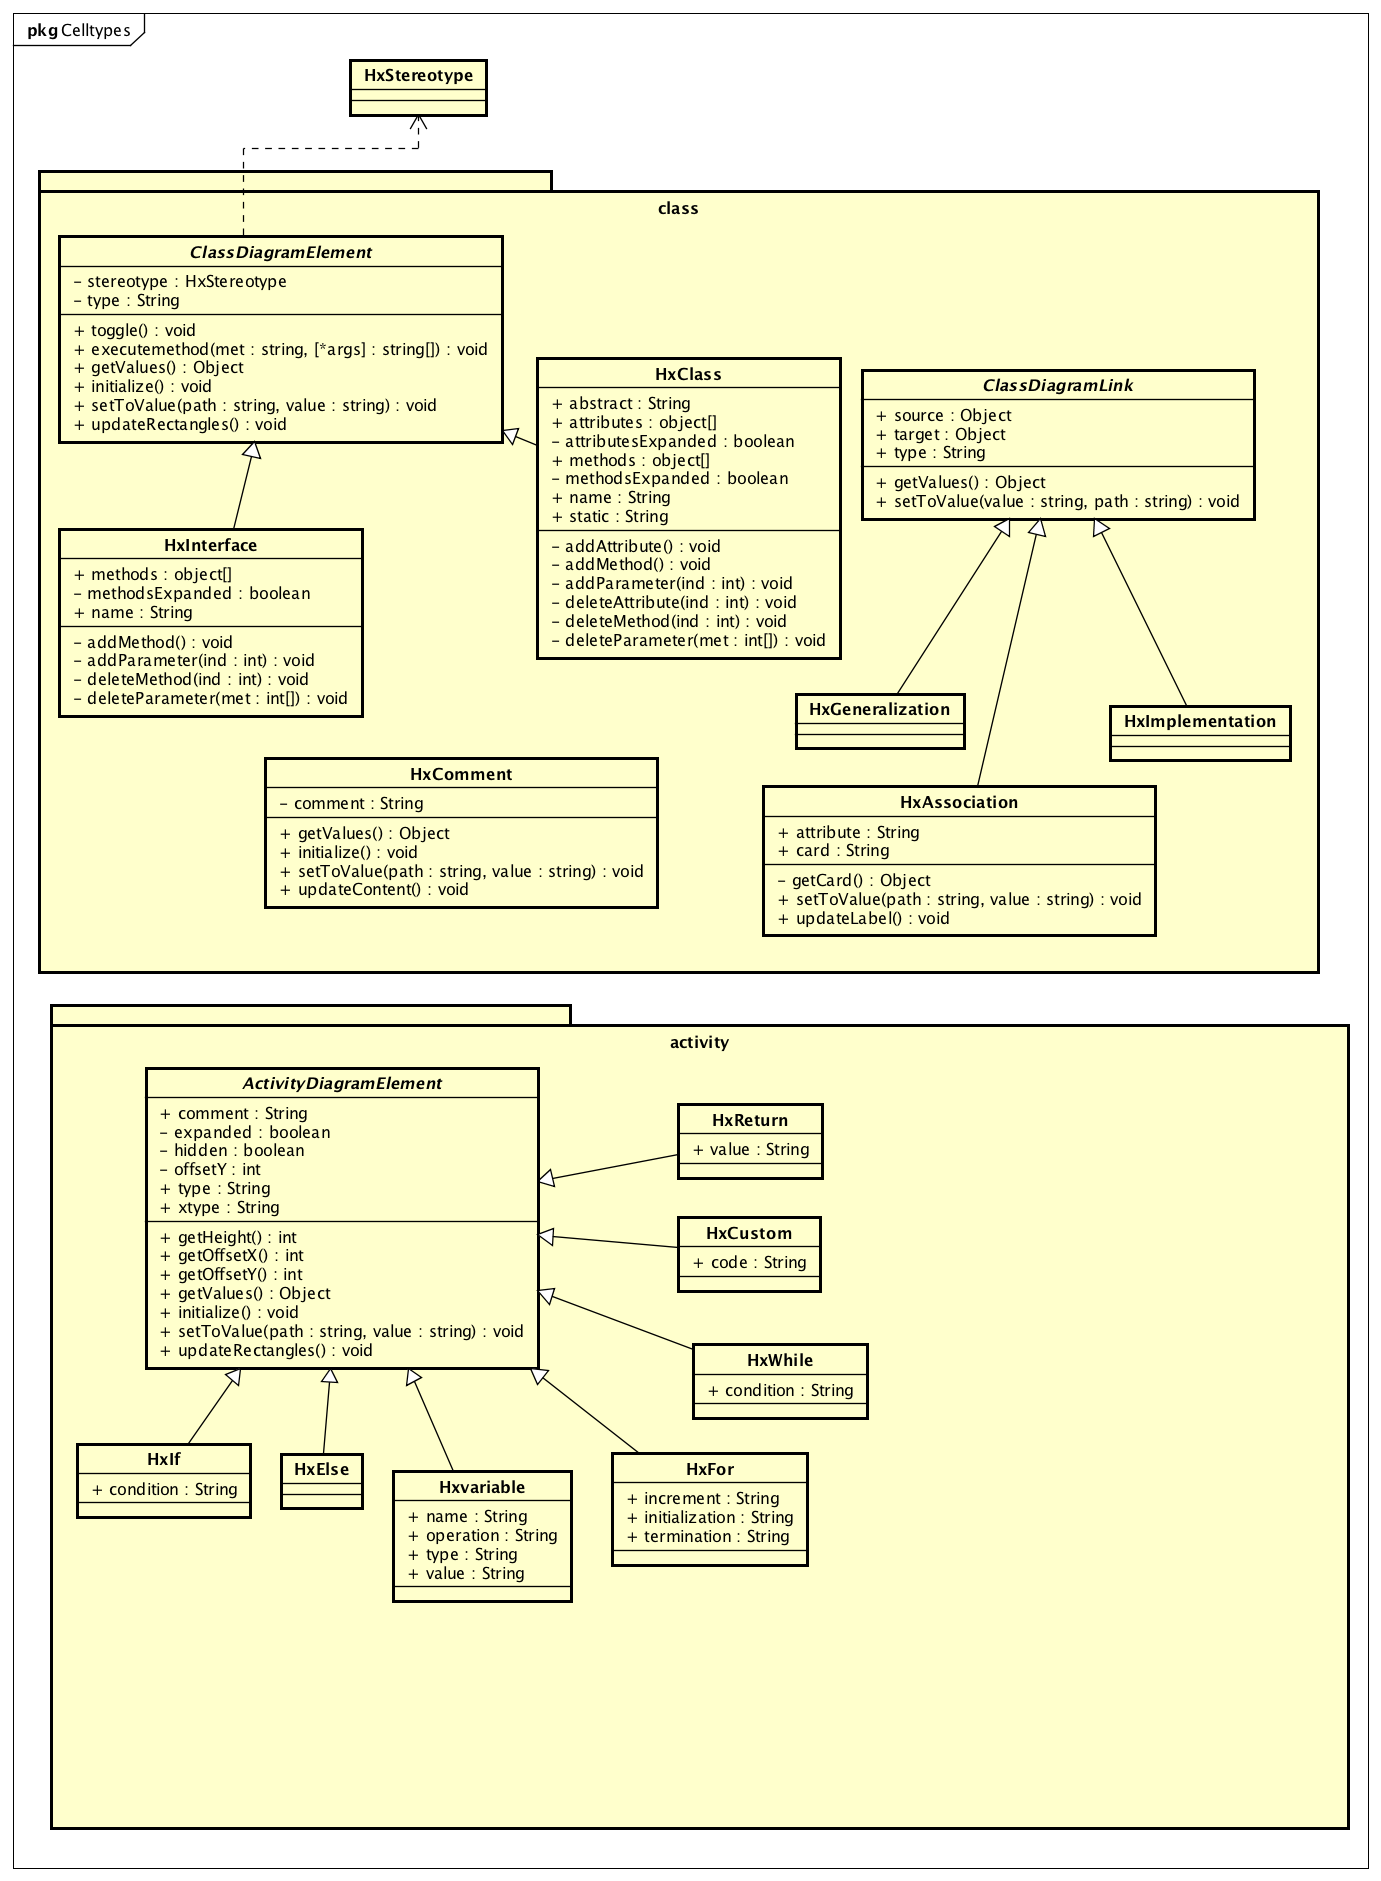
\includegraphics[scale=0.4,keepaspectratio]{img/client/celltypes_pkg.png}}
\caption{\nogloxy{swedesigner::client::celltypes}}
\end{figure}
\FloatBarrier
\begin{itemize}
\item \textbf{Descrizione}\\
Questo package contiene la definizione del modello degli elementi grafici dell'applicazione (e.g. diagrammi delle classi, blocchi condizionali\dots). 
\item \textbf{Padre}: \hyperref[\nogloxy{swedesigner::client::model}]{\nogloxy{\texttt{model}}}
\item \textbf{Package contenuti}:
\begin{itemize}
\item \hyperref[\nogloxy{swedesigner::client::model::celltypes::activity}]{\nogloxy{\texttt{activity}}}\\
Questo package contiene la definizione del modello degli elementi specifi del diagramma delle classi dell'applicazione.
\item \hyperref[\nogloxy{swedesigner::client::model::celltypes::class}]{\nogloxy{\texttt{class}}}\\
Questo package contiene la definizione del modello degli elementi specifi del diagramma delle classi dell'applicazione.
\end{itemize}
\end{itemize}
\subsubsection{Classi}
\subsubsubsection{\nogloxy{swedesigner::client::model::celltypes::HxStereotype}}
\label{\nogloxy{swedesigner::client::model::celltypes::HxStereotype}}
\begin{itemize}
\item \textbf{Descrizione}\\
questa classe rappresenta le caratteristiche dello stereotipo che viene assegnato ad un \texttt{ClassDiagramElement} come i meta-attributi e meta-metodi, i quali sono essere ridefiniti dalla classe o interfaccia implementata tramite \proj{}. 
\item \textbf{Utilizzo}\\
ogni elemento possiederà un unico stereotipo per semplificare l'implementazione di \proj{}. Gli stereotipi disponibili sono presenti all'interno della classe \texttt{ProjectStereotypes} (all'interno di \emph{model::utility}).
\item \textbf{Relazioni con altre classi}:
\begin{itemize}
\item \textit{IN} \hyperref[\nogloxy{swedesigner::client::model::celltypes::class::ClassDiagramElement}]{\nogloxy{\texttt{ClassDiagramElement}}}\\
questa classe è la base di tutte le classi che rappresentano gli elementi del diagramma delle classi.
\item \textit{IN} \hyperref[\nogloxy{swedesigner::client::model::utility::ProjectStereotypes}]{\nogloxy{\texttt{ProjectStereotypes}}}\\
questa classe contiene al suo interno i possibili stereotipi utilizzabili recuperati dal server in modo asincrono. Conterrà una lista di elementi \textt{HxStereotype}.
\end{itemize}
\end{itemize}
\subsection{\nogloxy{swedesigner::client::model::celltypes::activity}}
\label{\nogloxy{swedesigner::client::model::celltypes::activity}}
\subsubsection{Informazioni generali}
\begin{itemize}
\item \textbf{Descrizione}\\
Questo package contiene la definizione del modello degli elementi specifi del diagramma delle classi dell'applicazione.
\item \textbf{Padre}: \hyperref[\nogloxy{swedesigner::client::model::celltypes}]{\nogloxy{\texttt{celltypes}}}
\end{itemize}
\subsubsection{Classi}
\subsubsubsection{\nogloxy{swedesigner::client::model::celltypes::activity::ActivityDiagramElement}}
\label{\nogloxy{swedesigner::client::model::celltypes::activity::ActivityDiagramElement}}
\begin{itemize}
\item \textbf{Descrizione}\\
questa classe è la base di tutte le classi che rappresentano i blocchi del diagramma delle attività.
\item \textbf{Utilizzo}\\
estende sottotipi della classe \texttt{Element} (la quale deriva a sua volta da \texttt{Cell})  di \jointjs{} e viene estesa da tutte le classi specifiche di ogni blocco del diagramma delle attività. Questa classe è indirettamente correlata a \texttt{NewCellFactory}.
\item \textbf{Sottoclassi}:
\begin{itemize}
\item \hyperref[\nogloxy{swedesigner::client::model::celltypes::activity::HxCustom}]{\nogloxy{\texttt{HxCustom}}}
\item \hyperref[\nogloxy{swedesigner::client::model::celltypes::activity::HxElse}]{\nogloxy{\texttt{HxElse}}}
\item \hyperref[\nogloxy{swedesigner::client::model::celltypes::activity::HxFor}]{\nogloxy{\texttt{HxFor}}}
\item \hyperref[\nogloxy{swedesigner::client::model::celltypes::activity::HxIf}]{\nogloxy{\texttt{HxIf}}}
\item \hyperref[\nogloxy{swedesigner::client::model::celltypes::activity::HxReturn}]{\nogloxy{\texttt{HxReturn}}}
\item \hyperref[\nogloxy{swedesigner::client::model::celltypes::activity::HxVariable}]{\nogloxy{\texttt{HxVariable}}}
\item \hyperref[\nogloxy{swedesigner::client::model::celltypes::activity::HxWhile}]{\nogloxy{\texttt{HxWhile}}}
\end{itemize}
\item \textbf{Relazioni con altre classi}:
\begin{itemize}
\item \textit{OUT} \hyperref[\nogloxy{swedesigner::client::model::NewCellFactory}]{\nogloxy{\texttt{NewCellFactory}}}\\
questa classe si occupa di fornire un'istanza di una cella del tipo richiesto da \texttt{NewCellModel}. 
\end{itemize}
\item \textbf{Attributi}:
\begin{itemize}
\item \nogloxy{\texttt{# comment: string}}
\\ Questo attributo indica un commento che è possibile scrivere all'interno di ogni blocco
\item \nogloxy{\texttt{# expanded: bool}}
\\ Questo attributo indica se l'elemento è ridotto oppure è visibile per intero
\item \nogloxy{\texttt{# hidden: bool}}
\\ Questo attributo indica se la cella deve essere visualizzata
\item \nogloxy{\texttt{# offsetY: int}}
\\ Questo attributo indica quanto deve essere spostata la cella nel diagramma delle attività. Questo valore viene gestito da /texttt{ProjectView}
\item \nogloxy{\texttt{# type: string}}
\\ Questo attributo indica il tipo della cella,in modo  che questa possa essere identificata facilmente da chi la usa
\item \nogloxy{\texttt{# xtype: string}}
\\ Questo attributo indica il tipo della cella che verrà poi visualizzato. Verrà ridefinito da ogni classe che eredita questa
\end{itemize}
\item \textbf{Metodi}:
\begin{itemize}
\item \nogloxy{\texttt{+ getHeight(): int}}
\\ Questo metodo ritorna un valore che indica l'altezza di un blocco
\item \nogloxy{\texttt{+ getOffsetX(): int}}
\\ Questo metodo ritorna un valore che indica l'indentazione rispetto ai blocchi genitori
\item \nogloxy{\texttt{+ getOffsetY(): int}}
\\ Questo metodo ritorna il valore dell'attributo offsetY
\item \nogloxy{\texttt{+ getValues(): object}}
\\ Questo metodo si occupa di recuperare le proprietà di un blocco del diagramma delle attività
\item \nogloxy{\texttt{+ initialize(): void}}
\\ Questo metodo si occupa di inizializzare la classe
\item \nogloxy{\texttt{+ setToValue(path: string, value: string): void}}
\\ Questo metodo si occupa di impostare un attributo passato passato come parametro al valore scelto
\\ \textbf{Parametri}:
\begin{itemize}
\item \nogloxy{\texttt{path: string}}
\\ Questo parametro indica l'attributo da modificare
\item \nogloxy{\texttt{value: string}}
\\ Questo parametro indica il valore da assegnare
\end{itemize}
\item \nogloxy{\texttt{+ updateRectangles(): void}}
\\ Questo metodo si occupa di aggiornare degli elementi utili alla visualizzazione in base ai valori di attributi come expanded ed hidden
\end{itemize}
\end{itemize}

\subsubsubsection{\nogloxy{swedesigner::client::model::celltypes::activity::HxCustom}}
\label{\nogloxy{swedesigner::client::model::celltypes::activity::HxCustom}}
\begin{itemize}
\item \textbf{Descrizione}\\
questa classe rappresenta il blocco custom del diagramma delle attività che permette all'utente di inserire liberamente codice nel linguaggio target scelto.
\item \textbf{Utilizzo}\\
la classe \texttt{NewCellFactory} ritorna un'istanza di questa classe ogni volta che l'utente richiede un nuovo blocco di codice personalizzato.
\item \textbf{Classi ereditate}:
\begin{itemize}
\item \hyperref[\nogloxy{swedesigner::client::model::celltypes::activity::ActivityDiagramElement}]{\nogloxy{\texttt{ActivityDiagramElement}}}
\end{itemize}
\item \textbf{Attributi}:
\begin{itemize}
\item \nogloxy{\texttt{- code: string}}
\\ Questo attributo indica il blocco di codice custom che l'utente inserisce
\end{itemize}
\end{itemize}

\subsubsubsection{\nogloxy{swedesigner::client::model::celltypes::activity::HxElse}}
\label{\nogloxy{swedesigner::client::model::celltypes::activity::HxElse}}
\begin{itemize}
\item \textbf{Descrizione}\\
Questa classe rappresenta il blocco else del diagramma delle attività
\item \textbf{Utilizzo}\\
la classe \texttt{NewCellFactory} ritorna un'istanza di questa classe ogni volta che l'utente richiede un nuovo blocco \texttt{for}.
\item \textbf{Classi ereditate}:
\begin{itemize}
\item \hyperref[\nogloxy{swedesigner::client::model::celltypes::activity::ActivityDiagramElement}]{\nogloxy{\texttt{ActivityDiagramElement}}}
\end{itemize}
\end{itemize}

\subsubsubsection{\nogloxy{swedesigner::client::model::celltypes::activity::HxFor}}
\label{\nogloxy{swedesigner::client::model::celltypes::activity::HxFor}}
\begin{itemize}
\item \textbf{Descrizione}\\
questa classe rappresenta il blocco \texttt{for} del diagramma delle attività.
\item \textbf{Utilizzo}\\
la classe \texttt{NewCellFactory} ritorna un'istanza di questa classe ogni volta che l'utente richiede un nuovo blocco \texttt{for}.
\item \textbf{Classi ereditate}:
\begin{itemize}
\item \hyperref[\nogloxy{swedesigner::client::model::celltypes::activity::ActivityDiagramElement}]{\nogloxy{\texttt{ActivityDiagramElement}}}
\end{itemize}
\item \textbf{Attributi}:
\begin{itemize}
\item \nogloxy{\texttt{- increment: string}}
\\ Questo attributo indica la parte di incremento di un for
\item \nogloxy{\texttt{- initialization: string}}
\\ Questo attributo indica la parte di inizializzazione di un for
\item \nogloxy{\texttt{- termination: string}}
\\ Questo attributo indica la parte di terminazione di un for
\end{itemize}
\end{itemize}

\subsubsubsection{\nogloxy{swedesigner::client::model::celltypes::activity::HxIf}}
\label{\nogloxy{swedesigner::client::model::celltypes::activity::HxIf}}
\begin{itemize}
\item \textbf{Descrizione}\\
questa classe rappresenta il blocco \texttt{if} del diagramma delle attività.
\item \textbf{Utilizzo}\\
la classe \texttt{NewCellFactory} ritorna un'istanza di questa classe ogni volta che l'utente richiede un nuovo blocco \texttt{if}.
\item \textbf{Classi ereditate}:
\begin{itemize}
\item \hyperref[\nogloxy{swedesigner::client::model::celltypes::activity::ActivityDiagramElement}]{\nogloxy{\texttt{ActivityDiagramElement}}}
\end{itemize}
\item \textbf{Attributi}:
\begin{itemize}
\item \nogloxy{\texttt{- condition: string}}
\\ Questo attributo indica la condizione del blocco if
\end{itemize}
\end{itemize}

\subsubsubsection{\nogloxy{swedesigner::client::model::celltypes::activity::HxReturn}}
\label{\nogloxy{swedesigner::client::model::celltypes::activity::HxReturn}}
\begin{itemize}
\item \textbf{Descrizione}\\
questa classe rappresenta il blocco \emph{return} del diagramma delle attività.
\item \textbf{Utilizzo}\\
la classe \texttt{NewCellFactory} ritorna un'istanza di questa classe ogni volta che l'utente richiede un nuovo blocco \emph{return}.
\item \textbf{Classi ereditate}:
\begin{itemize}
\item \hyperref[\nogloxy{swedesigner::client::model::celltypes::activity::ActivityDiagramElement}]{\nogloxy{\texttt{ActivityDiagramElement}}}
\end{itemize}
\item \textbf{Attributi}:
\begin{itemize}
\item \nogloxy{\texttt{- value: string}}
\\ Questo attributo indica la stringa di ritorno del blocco return
\end{itemize}
\end{itemize}

\subsubsubsection{\nogloxy{swedesigner::client::model::celltypes::activity::HxVariable}}
\label{\nogloxy{swedesigner::client::model::celltypes::activity::HxVariable}}
\begin{itemize}
\item \textbf{Descrizione}\\
questa classe rappresenta il blocco di assegnazione o inizializzazione di una variabile o di chiamata di un metodo del diagramma delle attività.
\item \textbf{Utilizzo}\\
la classe \texttt{NewCellFactory} ritorna un'istanza di questa classe ogni volta che l'utente richiede un nuovo blocco variabile.
\item \textbf{Classi ereditate}:
\begin{itemize}
\item \hyperref[\nogloxy{swedesigner::client::model::celltypes::activity::ActivityDiagramElement}]{\nogloxy{\texttt{ActivityDiagramElement}}}
\end{itemize}
\item \textbf{Attributi}:
\begin{itemize}
\item \nogloxy{\texttt{- name: string}}
\\ Questo attributo indica il nome della variabile. È opzionale
\item \nogloxy{\texttt{- operation: string}}
\\ Questo attributo indica l'operazione da eseguire sulla variabile. È opzionale
\item \nogloxy{\texttt{- type: string}}
\\ Questo attributo indica il tipo della variabile. È opzionale
\item \nogloxy{\texttt{- value: string}}
\\ Questo attributo indica il valore che può essere un'inizializzazione,un'assegnazione od una chiamata ad un metodo. È opzionale
\end{itemize}
\end{itemize}

\subsubsubsection{\nogloxy{swedesigner::client::model::celltypes::activity::HxWhile}}
\label{\nogloxy{swedesigner::client::model::celltypes::activity::HxWhile}}
\begin{itemize}
\item \textbf{Descrizione}\\
questa classe rappresenta il blocco \emph{while} del diagramma delle attività.
\item \textbf{Utilizzo}\\
la classe \texttt{NewCellFactory} ritorna un'istanza di questa classe ogni volta che l'utente richiede un nuovo blocco \emph{while}.
\item \textbf{Classi ereditate}:
\begin{itemize}
\item \hyperref[\nogloxy{swedesigner::client::model::celltypes::activity::ActivityDiagramElement}]{\nogloxy{\texttt{ActivityDiagramElement}}}
\end{itemize}
\item \textbf{Attributi}:
\begin{itemize}
\item \nogloxy{\texttt{- condition: string}}
\\ Questo attributo rappresenta la condizione del while
\end{itemize}
\end{itemize}
\subsection{\nogloxy{swedesigner::client::model::celltypes::class}}
\label{\nogloxy{swedesigner::client::model::celltypes::class}}
\subsubsection{Informazioni generali}
\begin{itemize}
\item \textbf{Descrizione}\\
Questo package contiene la definizione del modello degli elementi specifi del diagramma delle classi dell'applicazione.
\item \textbf{Padre}: \hyperref[\nogloxy{swedesigner::client::model::celltypes}]{\nogloxy{\texttt{celltypes}}}
\end{itemize}
\subsubsection{Classi}
\subsubsubsection{\nogloxy{swedesigner::client::model::celltypes::class::ClassDiagramElement}}
\label{\nogloxy{swedesigner::client::model::celltypes::class::ClassDiagramElement}}
\begin{itemize}
\item \textbf{Descrizione}\\
questa classe è la base di tutte le classi che rappresentano gli elementi del diagramma delle classi.
\item \textbf{Utilizzo}\\
eredita da sottotipi della classe \texttt{Element} di \jointjs{} (la quale deriva a sua volta da \texttt{Cell}) e viene estesa da tutte le classi specifiche di ogni blocco del diagramma delle classi. Questa classe è indirettamente correlata con \texttt{NewCellFactory}, derivando da \texttt{Cell}.
\item \textbf{Sottoclassi}:
\begin{itemize}
\item \hyperref[\nogloxy{swedesigner::client::model::celltypes::class::HxClass}]{\nogloxy{\texttt{HxClass}}}
\item \hyperref[\nogloxy{swedesigner::client::model::celltypes::class::HxInterface}]{\nogloxy{\texttt{HxInterface}}}
\end{itemize}
\item \textbf{Relazioni con altre classi}:
\begin{itemize}
\item \textit{IN} \hyperref[\nogloxy{swedesigner::client::model::NewCellFactory}]{\nogloxy{\texttt{NewCellFactory}}}\\
questa classe si occupa di fornire un'istanza di una cella del tipo richiesto da \texttt{NewCellModel}. 
\item \textit{OUT} \hyperref[\nogloxy{swedesigner::client::model::celltypes::HxStereotype}]{\nogloxy{\texttt{HxStereotype}}}\\
questa classe rappresenta le caratteristiche dello stereotipo che viene assegnato ad un \texttt{ClassDiagramElement} come i meta-attributi e meta-metodi, i quali sono essere ridefiniti dalla classe o interfaccia implementata tramite \proj{}. 
\end{itemize}
\item \textbf{Attributi}:
\begin{itemize}
\item \nogloxy{\texttt{# type: string}}
\\ Questo attributo indica il tipo della cella,in modo che questa possa essere identificata facilmente da chi la usa
\end{itemize}
\item \textbf{Metodi}:
\begin{itemize}
\item \nogloxy{\texttt{+ executemethod(met: string, [*args]: string[]): void}}
\\ Questo metodo permette di eseguire un altro metodo della classe in base agli argomenti passati
\\ \textbf{Parametri}:
\begin{itemize}
\item \nogloxy{\texttt{met: string}}
\\ Questo parametro indica il nome del metodo da eseguire
\item \nogloxy{\texttt{[*args]: string[]}}
\\ Indica una serie di parametri da passare ai metodi chiamati
\end{itemize}
\item \nogloxy{\texttt{+ getValues(): object}}
\\ Questo metodo si occupa di recuperare le proprietà di un blocco del diagramma delle classi
\item \nogloxy{\texttt{+ initialize(): void}}
\\ Questo metodo si occupa di inizializzare la classe
\item \nogloxy{\texttt{+ setToValue(path: string, value: string): void}}
\\ Questo metodo si occupa di impostare un attributo passato come parametro al valore scelto
\\ \textbf{Parametri}:
\begin{itemize}
\item \nogloxy{\texttt{path: string}}
\\ Questo parametro indica l'attributo da modificare
\item \nogloxy{\texttt{value: string}}
\\ Questo parametro indica il valore da assegnare
\end{itemize}
\item \nogloxy{\texttt{+ updateRectangles(): void}}
\\ Questo metodo si occupa di aggiornare degli elementi utili alla visualizzazione della cella
\end{itemize}
\end{itemize}

\subsubsubsection{\nogloxy{swedesigner::client::model::celltypes::class::ClassDiagramLink}}
\label{\nogloxy{swedesigner::client::model::celltypes::class::ClassDiagramLink}}
\begin{itemize}
\item \textbf{Descrizione}\\
questa classe è la base di tutte le classi che rappresentano le relazioni tra gli elementi del diagramma delle classi.
\item \textbf{Utilizzo}\\
eredita dalla classe \texttt{Link} di \jointjs{} e viene estesa da tutte le classi specifiche di ogni relazione del diagramma delle classi.
\item \textbf{Sottoclassi}:
\begin{itemize}
\item \hyperref[\nogloxy{swedesigner::client::model::celltypes::class::HxAssociation}]{\nogloxy{\texttt{HxAssociation}}}
\item \hyperref[\nogloxy{swedesigner::client::model::celltypes::class::HxGeneralization}]{\nogloxy{\texttt{HxGeneralization}}}
\item \hyperref[\nogloxy{swedesigner::client::model::celltypes::class::HxImplementation}]{\nogloxy{\texttt{HxImplementation}}}
\end{itemize}
\item \textbf{Attributi}:
\begin{itemize}
\item \nogloxy{\texttt{# source: object}}
\\ Questo attributo indica la cella di partenza della relazione
\item \nogloxy{\texttt{# target: object}}
\\ Questo attributo indica la cella di destinazione della relazione
\item \nogloxy{\texttt{# type: string}}
\\ Questo attributo indica il tipo della relazione,in modo che questa possa essere identificata facilmente da chi la usa
\end{itemize}
\item \textbf{Metodi}:
\begin{itemize}
\item \nogloxy{\texttt{+ getValues(): object}}
\\ Questo metodo si occupa di recuperare le proprietà di una relazione
\item \nogloxy{\texttt{+ setToValue(value: string, path: string): void}}
\\ Questo metodo si occupa di impostare un attributo passato come parametro al valore scelto
\\ \textbf{Parametri}:
\begin{itemize}
\item \nogloxy{\texttt{value: string}}
\\ Questo parametro indica il valore nuovo per l'attributo
\item \nogloxy{\texttt{path: string}}
\\ Questo parametro indica l'attributo da modificare
\end{itemize}
\end{itemize}
\end{itemize}

\subsubsubsection{\nogloxy{swedesigner::client::model::celltypes::class::HxAssociation}}
\label{\nogloxy{swedesigner::client::model::celltypes::class::HxAssociation}}
\begin{itemize}
\item \textbf{Descrizione}\\
Questa classe rappresenta una relazione associazione tra due blocchi del diagramma delle classi
\item \textbf{Utilizzo}\\
eredita dalla classe \texttt{ClassDiagramLink}. È indirettamente collegata a \texttt{NewCellFactory} in quanto è anch'essa una derivata di \texttt{Cell}.
\item \textbf{Classi ereditate}:
\begin{itemize}
\item \hyperref[\nogloxy{swedesigner::client::model::celltypes::class::ClassDiagramLink}]{\nogloxy{\texttt{ClassDiagramLink}}}
\end{itemize}
\item \textbf{Attributi}:
\begin{itemize}
\item \nogloxy{\texttt{- attribute: string}}
\\ Questo attributo indica l'attributo associato alla relazione
\item \nogloxy{\texttt{- card: string}}
\\ Questo attributo indica la cardinalità della relazione
\end{itemize}
\item \textbf{Metodi}:
\begin{itemize}
\item \nogloxy{\texttt{- getCard(): object}}
\\ Questo attributo ritorna la cardinalità della relazione
\item \nogloxy{\texttt{+ setToValue(path: string, value: string): void}}
\\ Questo metodo si occupa di impostare un attributo passato come parametro al valore scelto

\textbf{Parametri}:
\begin{itemize}
\item \nogloxy{\texttt{path: string}}
\\ Questo parametro indica l'attributo da modificare

\item \nogloxy{\texttt{value: string}}
\\ Questo parametro indica il valore da assegnare

\end{itemize}
\item \nogloxy{\texttt{+ updateLabel(): void}}
\\ Questo metodo si occupa di aggiornare dei parametri utili per la visualizzazione
\end{itemize}
\end{itemize}

\subsubsubsection{\nogloxy{swedesigner::client::model::celltypes::class::HxClass}}
\label{\nogloxy{swedesigner::client::model::celltypes::class::HxClass}}
\begin{itemize}
\item \textbf{Descrizione}\\
questa classe rappresenta il blocco \texttt{class} del diagramma delle classi UML.
\item \textbf{Utilizzo}\\
la classe \texttt{NewCellFactory} ritorna un'istanza di questa classe ogni volta che l'utente richiede un nuovo elemento \emph{class}.
\item \textbf{Classi ereditate}:
\begin{itemize}
\item \hyperref[\nogloxy{swedesigner::client::model::celltypes::class::ClassDiagramElement}]{\nogloxy{\texttt{ClassDiagramElement}}}
\end{itemize}
\item \textbf{Attributi}:
\begin{itemize}
\item \nogloxy{\texttt{- abstract: string}}
\\ Questo attributo indica se la classe è astratta
\item \nogloxy{\texttt{- attributes: object[]}}
\\ Questo attributo indica l'array di attributi di una classe
\item \nogloxy{\texttt{- attributesExpanded: bool}}
\\ Questo attributo indica se il blocco dovrà visualizzare la sezione attributi per intero oppure ridotta
\item \nogloxy{\texttt{- methods: object[]}}
\\ Questo attributo indica l'array di metodi di una classe
\item \nogloxy{\texttt{- methodsExpanded: bool}}
\\ Questo attributo indica se il blocco dovrà visualizzare la sezione metodi per intero oppure ridotta
\item \nogloxy{\texttt{- name: string}}
\\ Questo attributo indica il nome della classe
\item \nogloxy{\texttt{- static: string}}
\\ Questo attributo indica se la classe è statica
\end{itemize}
\item \textbf{Metodi}:
\begin{itemize}
\item \nogloxy{\texttt{- addAttribute(): void}}
\\ Questo metodo aggiunge un attributo alla classe
\item \nogloxy{\texttt{- addMethod(): void}}
\\ Questo metodo aggiunge un metodo alla classe
\item \nogloxy{\texttt{- addParameter(ind: int): void}}
\\ Questo metodo inserisce un nuovo parametro al metodo alla posizione indicata
\\ \textbf{Parametri}:
\begin{itemize}
\item \nogloxy{\texttt{ind: int}}
\\ Questo parametro indica l'indice del metodo al quale si vuole aggiungere un nuovo parametro
\end{itemize}
\item \nogloxy{\texttt{- deleteAttribute(ind: int): void}}
\\ Questo metodo elimina un attributo in base all'indice passato come parametro
\\ \textbf{Parametri}:
\begin{itemize}
\item \nogloxy{\texttt{ind: int}}
\\ Questo parametro indica l'indice dell'attributo da rimuovere
\end{itemize}
\item \nogloxy{\texttt{- deleteMethod(ind: int): void}}
\\ Questo metodo elimina il metodo alla posizione descritta dall'indice passato come parametro
\\ \textbf{Parametri}:
\begin{itemize}
\item \nogloxy{\texttt{ind: int}}
\\ Questo parametro indica l'indice del metodo da rimuovere 
\end{itemize}
\item \nogloxy{\texttt{- deleteParameter(met: int[]): void}}
\\ Questo metodo cancella un parametro al metodo specificato
\\ \textbf{Parametri}:
\begin{itemize}
\item \nogloxy{\texttt{met: int[]}}
\\ Questo parametro indica gli indici utili per identificare il parametro da rimuovere
\end{itemize}
\end{itemize}
\end{itemize}

\subsubsubsection{\nogloxy{swedesigner::client::model::celltypes::class::HxComment}}
\label{\nogloxy{swedesigner::client::model::celltypes::class::HxComment}}
\begin{itemize}
\item \textbf{Descrizione}\\
questa classe rappresenta la cella di commento del diagramma delle classi UML. Eredita da un tipo base di jointjs.
\item \textbf{Utilizzo}\\
la classe \texttt{NewCellFactory} ritorna un'istanza di questa classe ogni volta che l'utente richiede un nuovo commento.
\item \textbf{Attributi}:
\begin{itemize}
\item \nogloxy{\texttt{- comment: string}}
\\ Questo attributo indica la il commento che verrà visualizzato da questo blocco
\item \nogloxy{\texttt{- type: string}}
\\ Questo attributo indica il tipo di questa classe in modo da essere riconosciuto facilmente
\end{itemize}
\item \textbf{Metodi}:
\begin{itemize}
\item \nogloxy{\texttt{+ getValues(): object}}
\\ Questo metodo si occupa di recuperare le proprietà del blocco
\item \nogloxy{\texttt{+ initialize(): void}}
\\ Questo metodo si occupa di inizializzare la classe

\item \nogloxy{\texttt{+ setToValue(path: string, value: string): void}}
\\ Questo metodo si occupa di impostare un attributo passato come parametro al valore scelto

\textbf{Parametri}:
\begin{itemize}
\item \nogloxy{\texttt{path: string}}
\\ Questo parametro indica l'attributo da modificare

\item \nogloxy{\texttt{value: string}}
\\ Questo parametro indica il valore da assegnare

\end{itemize}
\item \nogloxy{\texttt{+ updateContent(): void}}
\\ Questo metodo si occupa di aggiornare degli elementi utili alla visualizzazione della cella

\end{itemize}
\end{itemize}

\subsubsubsection{\nogloxy{swedesigner::client::model::celltypes::class::HxGeneralization}}
\label{\nogloxy{swedesigner::client::model::celltypes::class::HxGeneralization}}
\begin{itemize}
\item \textbf{Descrizione}\\
questa classe rappresenta la relazione di generalizzazione tra due celle del diagramma delle classi.
\item \textbf{Utilizzo}\\
eredita dalla classe \texttt{ClassDiagramLink}. È indirettamente collegata a \texttt{NewCellFactory} in quanto è anch'essa una derivata di \texttt{Cell}.
\item \textbf{Classi ereditate}:
\begin{itemize}
\item \hyperref[\nogloxy{swedesigner::client::model::celltypes::class::ClassDiagramLink}]{\nogloxy{\texttt{ClassDiagramLink}}}
\end{itemize}
\end{itemize}

\subsubsubsection{\nogloxy{swedesigner::client::model::celltypes::class::HxImplementation}}
\label{\nogloxy{swedesigner::client::model::celltypes::class::HxImplementation}}
\begin{itemize}
\item \textbf{Descrizione}\\
questa classe rappresenta la relazione di implementazione tra due celle del diagramma delle classi.
\item \textbf{Utilizzo}\\
eredita dalla classe \texttt{ClassDiagramLink}. È indirettamente collegata a \texttt{NewCellFactory} in quanto è anch'essa una derivata di \texttt{Cell}.
\item \textbf{Classi ereditate}:
\begin{itemize}
\item \hyperref[\nogloxy{swedesigner::client::model::celltypes::class::ClassDiagramLink}]{\nogloxy{\texttt{ClassDiagramLink}}}
\end{itemize}
\end{itemize}

\subsubsubsection{\nogloxy{swedesigner::client::model::celltypes::class::HxInterface}}
\label{\nogloxy{swedesigner::client::model::celltypes::class::HxInterface}}
\begin{itemize}
\item \textbf{Descrizione}\\
questa classe rappresenta il costrutto \emph{interface} del diagramma delle classi UML.
\item \textbf{Utilizzo}\\
la classe \texttt{NewCellFactory} ritorna un'istanza di questa classe ogni volta che l'utente richiede un nuovo elemento \emph{interface}.
\item \textbf{Classi ereditate}:
\begin{itemize}
\item \hyperref[\nogloxy{swedesigner::client::model::celltypes::class::ClassDiagramElement}]{\nogloxy{\texttt{ClassDiagramElement}}}
\end{itemize}
\item \textbf{Attributi}:
\begin{itemize}
\item \nogloxy{\texttt{- methods: object[]}}
\\ Questo attributo indica l'array di metodi di una interfaccia
\item \nogloxy{\texttt{- methodsExpanded: bool}}
\\ Questo attributo indica se il blocco dovrà visualizzare la sezione metodi per intero oppure ridotta

\item \nogloxy{\texttt{+ name: string}}
\\ Questo attributo indica il nome dell'interfaccia

\end{itemize}
\item \textbf{Metodi}:
\begin{itemize}
\item \nogloxy{\texttt{- addMethod(): void}}
\\ Questo metodo aggiunge un metodo all'interfaccia
\item \nogloxy{\texttt{- addParameter(ind: int): void}}
\\ Questo metodo inserisce un nuovo parametro al metodo alla posizione indicata

\textbf{Parametri}:
\begin{itemize}
\item \nogloxy{\texttt{ind: int}}
\\ Questo parametro indica l'indice del metodo al quale si vuole aggiungere un nuovo parametro

\end{itemize}
\item \nogloxy{\texttt{- deleteMethod(ind: int): void}}
\\ Questo metodo elimina il metodo alla posizione descritta dall'indice passato come parametro

\textbf{Parametri}:
\begin{itemize}
\item \nogloxy{\texttt{ind: int}}
\\ Questo parametro indica l'indice del metodo da rimuovere

\end{itemize}
\item \nogloxy{\texttt{- deleteParameter(met: int[]): void}}
\\ Questo metodo cancella un parametro al metodo specificato

\textbf{Parametri}:
\begin{itemize}
\item \nogloxy{\texttt{met: int[]}}
\\ Questo parametro indica gli indici utili per identificare il parametro da rimuovere

\end{itemize}
\end{itemize}
\end{itemize}
\subsection{\nogloxy{swedesigner::client::model::utility}}
\label{\nogloxy{swedesigner::client::model::utility}}
\subsubsection{Informazioni generali}
\begin{itemize}
\item \textbf{Descrizione}\\
Questo package racchiude le classi che definiscono i principali comandi dell'applicazione; esse fanno parte di un unico pattern Command, usato dalla \texttt{AppView} principale.
\item \textbf{Padre}: \hyperref[\nogloxy{swedesigner::client::model}]{\nogloxy{\texttt{model}}}
\end{itemize}
\subsubsection{Classi}
\subsubsubsection{\nogloxy{swedesigner::client::model::utility::ProjectStereotypes}}
\label{\nogloxy{swedesigner::client::model::utility::ProjectStereotypes}}
\begin{itemize}
\item \textbf{Descrizione}\\
questa classe contiene al suo interno i possibili stereotipi utilizzabili recuperati dal server in modo asincrono. Conterrà una lista di elementi \textt{HxStereotype}.
\item \textbf{Utilizzo}\\
\texttt{DetailsView} necessita degli stereotipi esistenti per permettere l'inserimento e la modifica dello stereotipo di una classe. È possibile che la \texttt{NewCellFactory} faccia una richiesta simile a questa classe, al fine di poter fornire all'utente la possibilità di inserire una classe già stereotipata. 
\item \textbf{Relazioni con altre classi}:
\begin{itemize}
\item \textit{IN} \hyperref[\nogloxy{swedesigner::client::view::DetailsView}]{\nogloxy{\texttt{DetailsView}}}\\
questa classe si occupa di visualizzare tutti i campi di un blocco o di una relazione (come il nome di una classe, i suoi attributi, la condizione di un blocco \texttt{if} o il blocco di partenza di una relazione) permettendone anche la modifica. È possibile anche specificare uno stereotipo per la classe.

\item \textit{OUT} \hyperref[\nogloxy{swedesigner::client::model::celltypes::HxStereotype}]{\nogloxy{\texttt{HxStereotype}}}\\
questa classe rappresenta le caratteristiche dello stereotipo che viene assegnato ad un \texttt{ClassDiagramElement} come i meta-attributi e meta-metodi, i quali sono essere ridefiniti dalla classe o interfaccia implementata tramite \proj{}. 
\end{itemize}
\end{itemize}
\subsection{\nogloxy{swedesigner::client::view}}
\label{\nogloxy{swedesigner::client::view}}
\subsubsection{Informazioni generali}
\begin{figure}[h]
\centering
\nogloxy{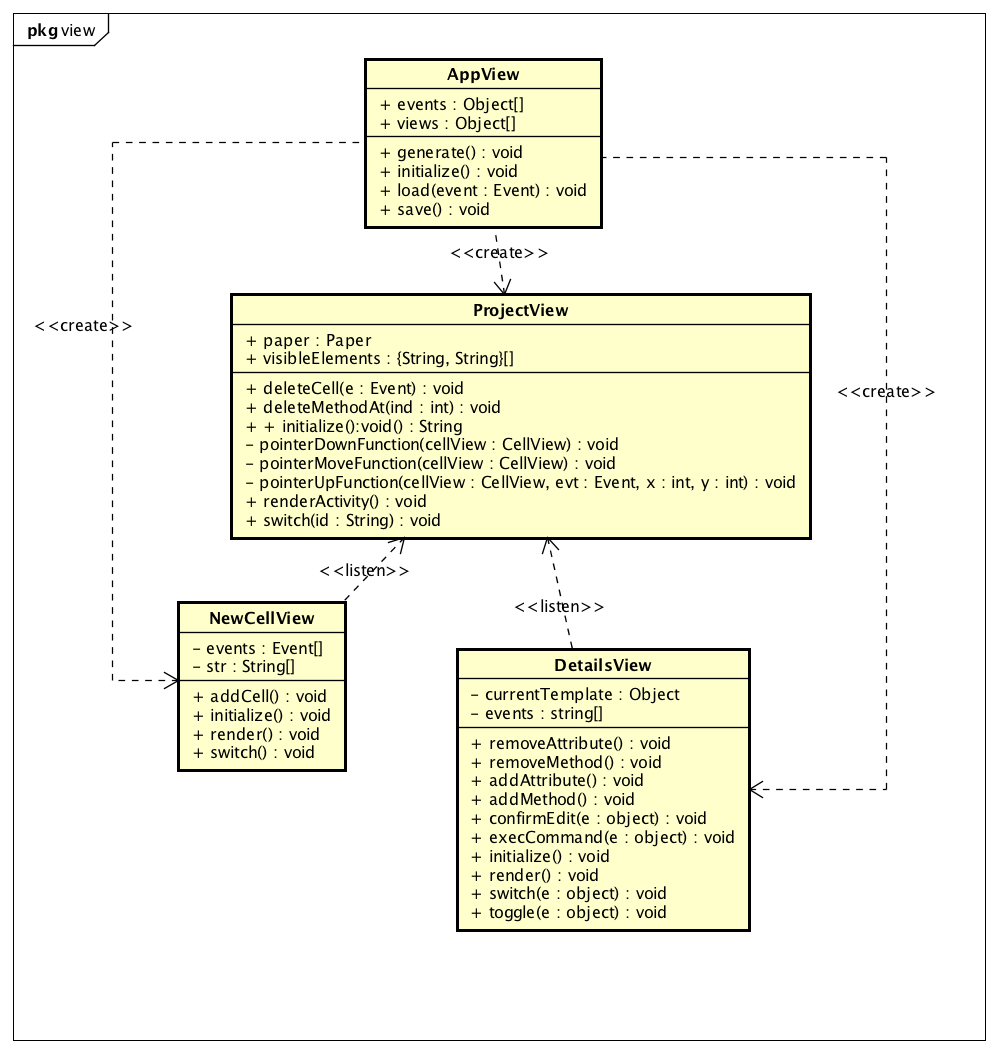
\includegraphics[scale=0.4,keepaspectratio]{img/client/view_pkg.png}}
\caption{\nogloxy{swedesigner::client::view}}
\end{figure}
\FloatBarrier
\begin{itemize}
\item \textbf{Descrizione}\\
Questo package raccoglie le classi che rappresentano i menù laterali e il \texttt{canvas} visualizzati dal browser, che popolano template e si sottoscrivono alla view tramite un pattern Observer. (I template non sono contenuti in questo package.)
\item \textbf{Padre}: \hyperref[\nogloxy{swedesigner::client}]{\nogloxy{\texttt{client}}}
\end{itemize}
\subsubsection{Classi}
\subsubsubsection{\nogloxy{swedesigner::client::view::AppView}}
\label{\nogloxy{swedesigner::client::view::AppView}}
\begin{itemize}
\item \textbf{Descrizione}\\
questa classe si occupa di gestire l'intera view dell'applicazione, componendo l'interfaccia principale e richiamando le altre view tramite il sistema a template di \backbonejs{}.
\item \textbf{Utilizzo}\\
essa è la prima classe costruita dall'entry point del programma.
\item \textbf{Relazioni con altre classi}:
\begin{itemize}
\item \textit{OUT} \hyperref[\nogloxy{swedesigner::client::model::ProjectCommand}]{\nogloxy{\texttt{ProjectCommand}}}\\
questa interfaccia descrive la struttura di un comando che viene chiamato da \texttt{AppView} quando l'utente decide di creare un nuovo progetto, di caricarne uno esistente, di salvarlo o di generare il codice dal diagramma. Il pattern realizzato è il pattern Command.
\item \textit{OUT} \hyperref[\nogloxy{swedesigner::client::model::ProjectModel}]{\nogloxy{\texttt{ProjectModel}}}\\
questa classe ci permette di aggiungere della logica alla collezione di tutti i diagrammi che possediamo.
\item \textit{OUT} \hyperref[\nogloxy{swedesigner::client::view::DetailsView}]{\nogloxy{\texttt{DetailsView}}}\\
questa classe si occupa di visualizzare tutti i campi di un blocco o di una relazione (come il nome di una classe, i suoi attributi, la condizione di un blocco \texttt{if} o il blocco di partenza di una relazione) permettendone anche la modifica. È possibile anche specificare uno stereotipo per la classe.

\item \textit{OUT} \hyperref[\nogloxy{swedesigner::client::view::NewCellView}]{\nogloxy{\texttt{NewCellView}}}\\
questa classe si occupa di visualizzare tutti i possibili blocchi e relazioni che si possono inserire nel diagramma delle classi o delle attività.
\item \textit{OUT} \hyperref[\nogloxy{swedesigner::client::view::ProjectView}]{\nogloxy{\texttt{ProjectView}}}\\
questa classe rappresenta l'area di disegno principale dell'applicazione, che necessita di essere cambiata tra diagramma delle classi e diagramma delle attività. 
\end{itemize}
\item \textbf{Attributi}:
\begin{itemize}
\item \nogloxy{\texttt{- events: Object[]}}
\\ Contiene gli eventi definiti, usando Backbone.js per la loro gestione.
\item \nogloxy{\texttt{- views: Object[]}}
\\ Contiene le view create da AppView.
\begin{itemize}
\item project (\emph{ProjectView})
\item details (\emph{DetailsView})
\item newCell (\emph{NewCellView})
\end{itemize}

\end{itemize}
\item \textbf{Metodi}:
\begin{itemize}
\item \nogloxy{\texttt{+ generate(): void}}
\\ Richiama il comando di caricamento progetto al server e generazione eseguibile.
\item \nogloxy{\texttt{+ initialize(): void}}
\\ Inizializza le corrette view dell'applicazione.
\item \nogloxy{\texttt{+ load(event: Event): void}}
\\ Richiama il comando di caricamento progetto da disco.
\\ \textbf{Parametri}:
\begin{itemize}
\item \nogloxy{\texttt{event: Event}}
\\ Evento che ha innescato l'azione.
\end{itemize}
\item \nogloxy{\texttt{+ save(): void}}
\\ Richiama il comando di salvataggio progetto.
\end{itemize}
\end{itemize}

\subsubsubsection{\nogloxy{swedesigner::client::view::DetailsView}}
\label{\nogloxy{swedesigner::client::view::DetailsView}}
\begin{itemize}
\item \textbf{Descrizione}\\
questa classe si occupa di visualizzare tutti i campi di un blocco o di una relazione (come il nome di una classe, i suoi attributi, la condizione di un blocco \texttt{if} o il blocco di partenza di una relazione) permettendone anche la modifica. È possibile anche specificare uno stereotipo per la classe.

\item \textbf{Utilizzo}\\
utilizza come model una tra le classi contenute nel package \texttt{celltypes}, in base alla selezione fatta dall'utente, e ne modifica i campi in base all'input. Essa eredita dalla \texttt{View} di \emph{Backbone.js} ed è una \emph{view} parallela alla \texttt{CellView} di ogni \texttt{Cell}, in quanto usa gli stessi modelli mostrando diversamente i dati.
In futuro, qualora l'implementazione di questa classe risulti troppo pesante o complicata da testare, è possibile subclassare questa classe in \emph{view} multiple e prevedere una nuova \emph{factory} di view.
\item \textbf{Relazioni con altre classi}:
\begin{itemize}
\item \textit{IN} \hyperref[\nogloxy{swedesigner::client::view::AppView}]{\nogloxy{\texttt{AppView}}}\\
questa classe si occupa di gestire l'intera view dell'applicazione, componendo l'interfaccia principale e richiamando le altre view tramite il sistema a template di \backbonejs{}.
\item \textit{OUT} \hyperref[\nogloxy{swedesigner::client::model::utility::ProjectStereotypes}]{\nogloxy{\texttt{ProjectStereotypes}}}\\
questa classe contiene al suo interno i possibili stereotipi utilizzabili recuperati dal server in modo asincrono. Conterrà una lista di elementi \textt{HxStereotype}.
\end{itemize}
\item \textbf{Attributi}:
\begin{itemize}
\item \nogloxy{\texttt{- currentTemplate: object}}
\\ Questo attributo indica il template corrente da utilizzare per visualizzare \texttt{detailsViews}
\item \nogloxy{\texttt{- events: string[]}}
\\ Questo attributo rappresenta gli eventi intercettati e gestiti dalla view
\end{itemize}
\item \textbf{Metodi}:
\begin{itemize}
\item \nogloxy{\texttt{+ confirmEdit(e: object): void}}
\\ Questo metodo chiama il metodo setToValue del modello in modo da modificare i valori di esso in base all'input
\\ \textbf{Parametri}:
\begin{itemize}
\item \nogloxy{\texttt{e: object}}
\\ Questo oggetto rappresenta un evento di un elemento html che contiene anche i valori presi in input dall'utente
\end{itemize}
\item \nogloxy{\texttt{+ execCommand(e: object): void}}
\\ Questo metodo si occupa di eseguire un metodo del modello(come ad esempio aggiunta o eliminazione attributi) in base al nome dell'elemento passato in input
\\ \textbf{Parametri}:
\begin{itemize}
\item \nogloxy{\texttt{e: object}}
\\ Questo parametro rappresenta un oggetto evento di un elemento html
\end{itemize}
\item \nogloxy{\texttt{+ initialize(): void}}
\\ Questo metodo si occupa di istanziare la classe e di metterla in ascolto dell'evento di cambio della cella selezionata
\item \nogloxy{\texttt{+ render(): void}}
\\ Questo metodo si occupa di visualizzare la view all'interno di un div in base all'attributo. \texttt{currentTemplate}
\item \nogloxy{\texttt{+ switch(e: object): void}}
\\ Questo metodo si occupa di chiamare il cambio di diagramma in base all'input
\\ \textbf{Parametri}:
\begin{itemize}
\item \nogloxy{\texttt{e: object}}
\\ Questo parametro indica un oggetto evento che contiene informazioni sull'oggetto html cliccato e l'id del metodo del quale si vuole aprire il relativo diagramma delle attività
\end{itemize}
\item \nogloxy{\texttt{+ toggle(e: object): void}}
\\ Questo metodo di occupa di modificare la visibilità dell'elemento passato in input
\\ \textbf{Parametri}:
\begin{itemize}
\item \nogloxy{\texttt{e: object}}
\\ Questo parametro rappresenta un evento click contentente informazioni sull'elemento che ha scatenato l'evento
\end{itemize}
\end{itemize}
\end{itemize}

\subsubsubsection{\nogloxy{swedesigner::client::view::NewCellView}}
\label{\nogloxy{swedesigner::client::view::NewCellView}}
\begin{itemize}
\item \textbf{Descrizione}\\
questa classe si occupa di visualizzare tutti i possibili blocchi e relazioni che si possono inserire nel diagramma delle classi o delle attività.
\item \textbf{Utilizzo}\\
utilizza \texttt{NewCellModel} per recuperare i blocchi e relazioni inseribili nel diagramma corrente (che può essere o delle classi o delle attività).
\item \textbf{Relazioni con altre classi}:
\begin{itemize}
\item \textit{IN} \hyperref[\nogloxy{swedesigner::client::view::AppView}]{\nogloxy{\texttt{AppView}}}\\
questa classe si occupa di gestire l'intera view dell'applicazione, componendo l'interfaccia principale e richiamando le altre view tramite il sistema a template di \backbonejs{}.
\item \textit{OUT} \hyperref[\nogloxy{swedesigner::client::model::NewCellModel}]{\nogloxy{\texttt{NewCellModel}}}\\
questa classe si occupa di fornire tutti i tipi di cell (tutti i blocchi e relazioni) da poter inserire nel diagramma corrente (o classi o attività).
\end{itemize}
\item \textbf{Attributi}:
\begin{itemize}
\item \nogloxy{\texttt{- events: Event[]}}
\\ Coppie chiave-valore usate da \backbonejs{} per la gestione degli eventi.
\item \nogloxy{\texttt{- str: String[]}}
\\ Rappresenta una lista di String che contiene i componenti HTML da inserire all'interno del DOM. Ogni stringa rappresenta un elemento che può essere inserito nel diagramma corrente.
\end{itemize}
\item \textbf{Metodi}:
\begin{itemize}
\item \nogloxy{\texttt{+ addCell(): void}}
\\ Richiama il metodo \emph{addCell} del proprio \emph{model} in modo da aggiungere una cella.
\item \nogloxy{\texttt{+ initialize(): void}}
\\ Assegna l'opportuno model alla view appena inizializzata e si mette in ascolto dei corretti eventi.
\item \nogloxy{\texttt{+ render(): void}}
\\ Genera all'interno del DOM codice HTML corretto per inserire tutte le possibili celle creabili. 
\item \nogloxy{\texttt{+ switch(): void}}
\\ Richiama il metodo \emph{switchComponents} del rispettivo model.
\end{itemize}
\end{itemize}

\subsubsubsection{\nogloxy{swedesigner::client::view::ProjectView}}
\label{\nogloxy{swedesigner::client::view::ProjectView}}
\begin{itemize}
\item \textbf{Descrizione}\\
questa classe rappresenta l'area di disegno principale dell'applicazione, che necessita di essere cambiata tra diagramma delle classi e diagramma delle attività. 
\item \textbf{Utilizzo}\\
seleziona l'elemento \emph{Graph} da visualizzare. esso è presente nel relativo \emph{model}, che sarà di volta in volta cambiato selezionandolo dalla sua \emph{collection}.
\item \textbf{Relazioni con altre classi}:
\begin{itemize}
\item \textit{IN} \hyperref[\nogloxy{swedesigner::client::view::AppView}]{\nogloxy{\texttt{AppView}}}\\
questa classe si occupa di gestire l'intera view dell'applicazione, componendo l'interfaccia principale e richiamando le altre view tramite il sistema a template di \backbonejs{}.
\item \textit{OUT} \hyperref[\nogloxy{swedesigner::client::model::ProjectModel}]{\nogloxy{\texttt{ProjectModel}}}\\
questa classe ci permette di aggiungere della logica alla collezione di tutti i diagrammi che possediamo.
\end{itemize}
\item \textbf{Attributi}:
\begin{itemize}
\item \nogloxy{\texttt{- paper: Paper}}
\\ Rappresenta l'area di disegno principale, contenuta nell'elemento HTML \emph{\#paper}.
All'interno di questo oggetto di \jointjs{} sono presenti alcuni elementi aggiuntivi.
\item \nogloxy{\texttt{- visibleElements: {String, String}[]}}
\\ Contiene le variabili e i metodi visibili all'interno dello scope selezionato. Nell'implementazione corrente, a seguito dell'incontro [RIFERIMENTO] con il committente, è stato deciso di non implementare completamente tali funzionalità, tuttavia mantenendo la possibilità di una futura implementazione; nel caso specifico, sarà implementata solo la visibilità degli attributi e metodi presenti nella classe corrente.
\end{itemize}
\item \textbf{Metodi}:
\begin{itemize}
\item \nogloxy{\texttt{+ deleteCell(e: Event): void}}
\\ Esegue la cancellazione di una cella da un diagramma tramite il tasto \emph{Canc}.

\textbf{Parametri}:
\begin{itemize}
\item \nogloxy{\texttt{e: Event}}
\\ L'evento che ha scatenato questo metodo.
\end{itemize}
\item \nogloxy{\texttt{+ deleteMethodAt(ind: int): void}}
\\ Cancella un diagramma dei metodi.	

\textbf{Parametri}:
\begin{itemize}
\item \nogloxy{\texttt{ind: int}}
\\ Indice del metodo da rimuovere.

\end{itemize}
\item \nogloxy{\texttt{+ getCurrentDiagramType(): String}}
\\ Ritorna una stringa che rappresenta il tipo di diagramma corrente.	

\item \nogloxy{\texttt{+ initialize(): void}}
\\ Inizializza i seguenti elementi: \begin{itemize} \item \emph{model} con un nuovo \emph{ProjectModel} \item \emph{paper} con un nuovo \emph{joint.dia.Paper} \end{itemize} Inoltre si occupa di collegare i seguenti eventi di \jointjs{} alle relative funzioni: \begin{itemize} \item \emph{cell:pointerup} e \emph{pointerUpFunction} \item \emph{cell:pointermove} e \emph{pointerMoveFunction} \item \emph{cell:pointerdown} e \emph{pointerDownFunction} \end{itemize} Infine esso ascolta l'evento \emph{renderActivity} per chiamare l'omonima funzione.	

\item \nogloxy{\texttt{- pointerDownFunction(cellView: CellView): void}}
\\ Gestisce il drag di una cella da parte di un utente.
\\ \textbf{Parametri}:
\begin{itemize}
\item \nogloxy{\texttt{cellView: CellView}}
\\ View della cella selezionata.
\end{itemize}
\item \nogloxy{\texttt{- pointerMoveFunction(cellView: CellView): void}}
\\ Gestisce il movimento del mouse da parte dell'utente durante un drag\&drop, evidenziando la cella in cui sarà inserita la cella che l'utente sta strascinando.	

\textbf{Parametri}:
\begin{itemize}
\item \nogloxy{\texttt{cellView: CellView}}
\\ View della cella trascinata.

\end{itemize}
\item \nogloxy{\texttt{- pointerUpFunction(cellView: CellView, evt: Event, x: int, y: int): void}}
\\ Gestisce il drop di una cella, occupandosi delle seguenti operazioni: \begin{itemize} \item Spostamento della cella in una nuova posizione \item Spostamento dei figli della cella nella nuova posizione (corretta) \item Operazioni di cambiamento del padre \item Aggiornare nuovamente l'area di disegno \end{itemize} Si lascia all'implementatore la possibilità di spezzare questo metodo in più componenti, nel caso questo risulti complicato da sviluppare e da testare.	

\textbf{Parametri}:
\begin{itemize}
\item \nogloxy{\texttt{cellView: CellView}}
\\ View della cella selezionata.
\item \nogloxy{\texttt{evt: Event}}
\\ Rappresenta l'evento da cui è chiamato.
\item \nogloxy{\texttt{x: int}}
\\ Coordinata \emph{x} del puntatore quando rilasciato.
\item \nogloxy{\texttt{y: int}}
\\ Coordinata \emph{y} del puntatore quando rilasciato.
\end{itemize}
\item \nogloxy{\texttt{+ renderActivity(): void}}
\\ Aggiorna l'area di disegno posizionando correttamente sullo schermo i blocchi del diagramma delle attività. Sfrutta \emph{offsetY}, \emph{hidden}, \emph{expanded} di ogni blocco.	

\item \nogloxy{\texttt{+ switch(id: String): void}}
\\ Si occupa di cambiare il diagramma corrente.	

\textbf{Parametri}:
\begin{itemize}
\item \nogloxy{\texttt{id: String}}
\\ Id del diagramma da cambiare.
\end{itemize}
\end{itemize}
\end{itemize}
